\appendix
\section{Figures at full size}
\label{app:figures}

This appendix reproduces every figure from the report at full size for
readability. Each subsection corresponds to the source figure in the
body. Cross-references are bidirectional: the section figures point
here, and each appendix subsection notes which body figure it expands.

\subsection{Control architecture}
\label{app:arch}
\textit{(expansion of Fig.~\ref{fig:simulink_top_level} in §\ref{sec:architecture})}

\begin{figure}[H]
    \centering
    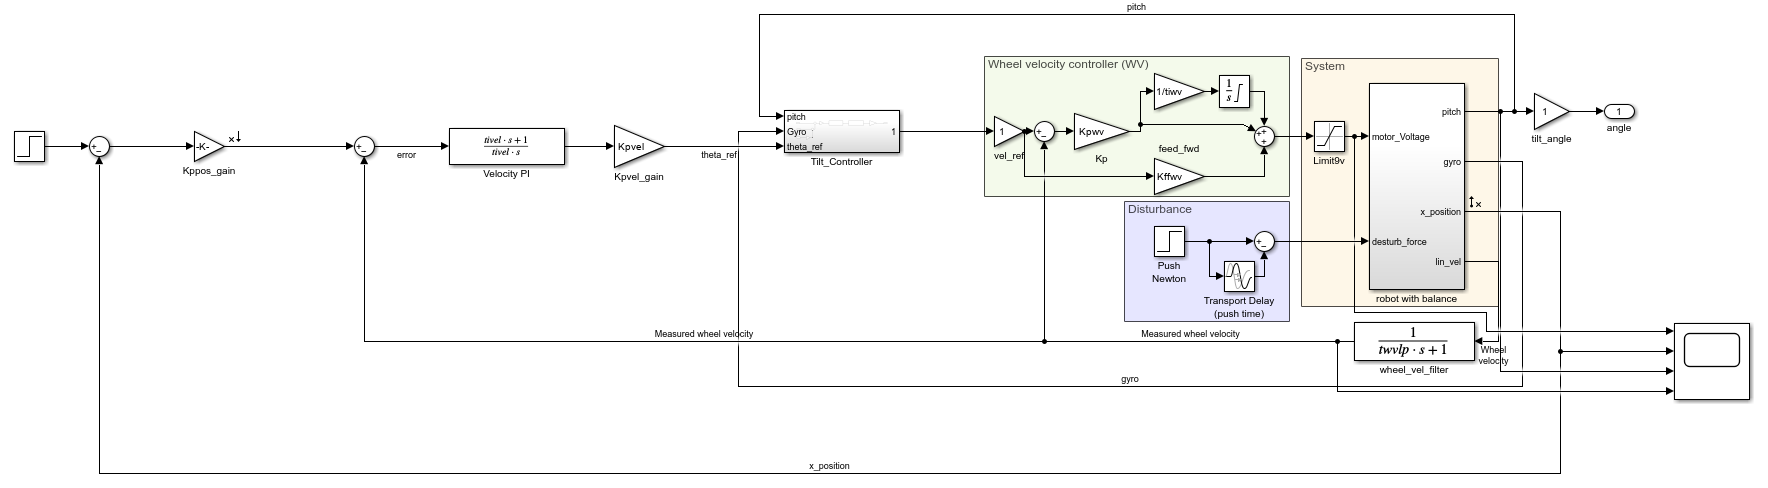
\includegraphics[width=\linewidth]{images/regbot_simulink_model.png}
    \caption{Top-level Simulink model. Left to right: position gain $K_{p,pos}$, velocity PI, the \texttt{Tilt\_Controller} subsystem (§\ref{sec:balance}), wheel-velocity PI with feed-forward, $\pm 9\,\mathrm{V}$ limiter, and the \texttt{robot with balance} Simscape Multibody plant.}
    \label{fig:app-arch}
\end{figure}

\subsection{Task 1 -- Wheel-speed verification}
\label{app:task1}
\textit{(expansion of Fig.~\ref{fig:task1-verify} in §\ref{sec:wheel-speed})}

\begin{figure}[H]
    \centering
    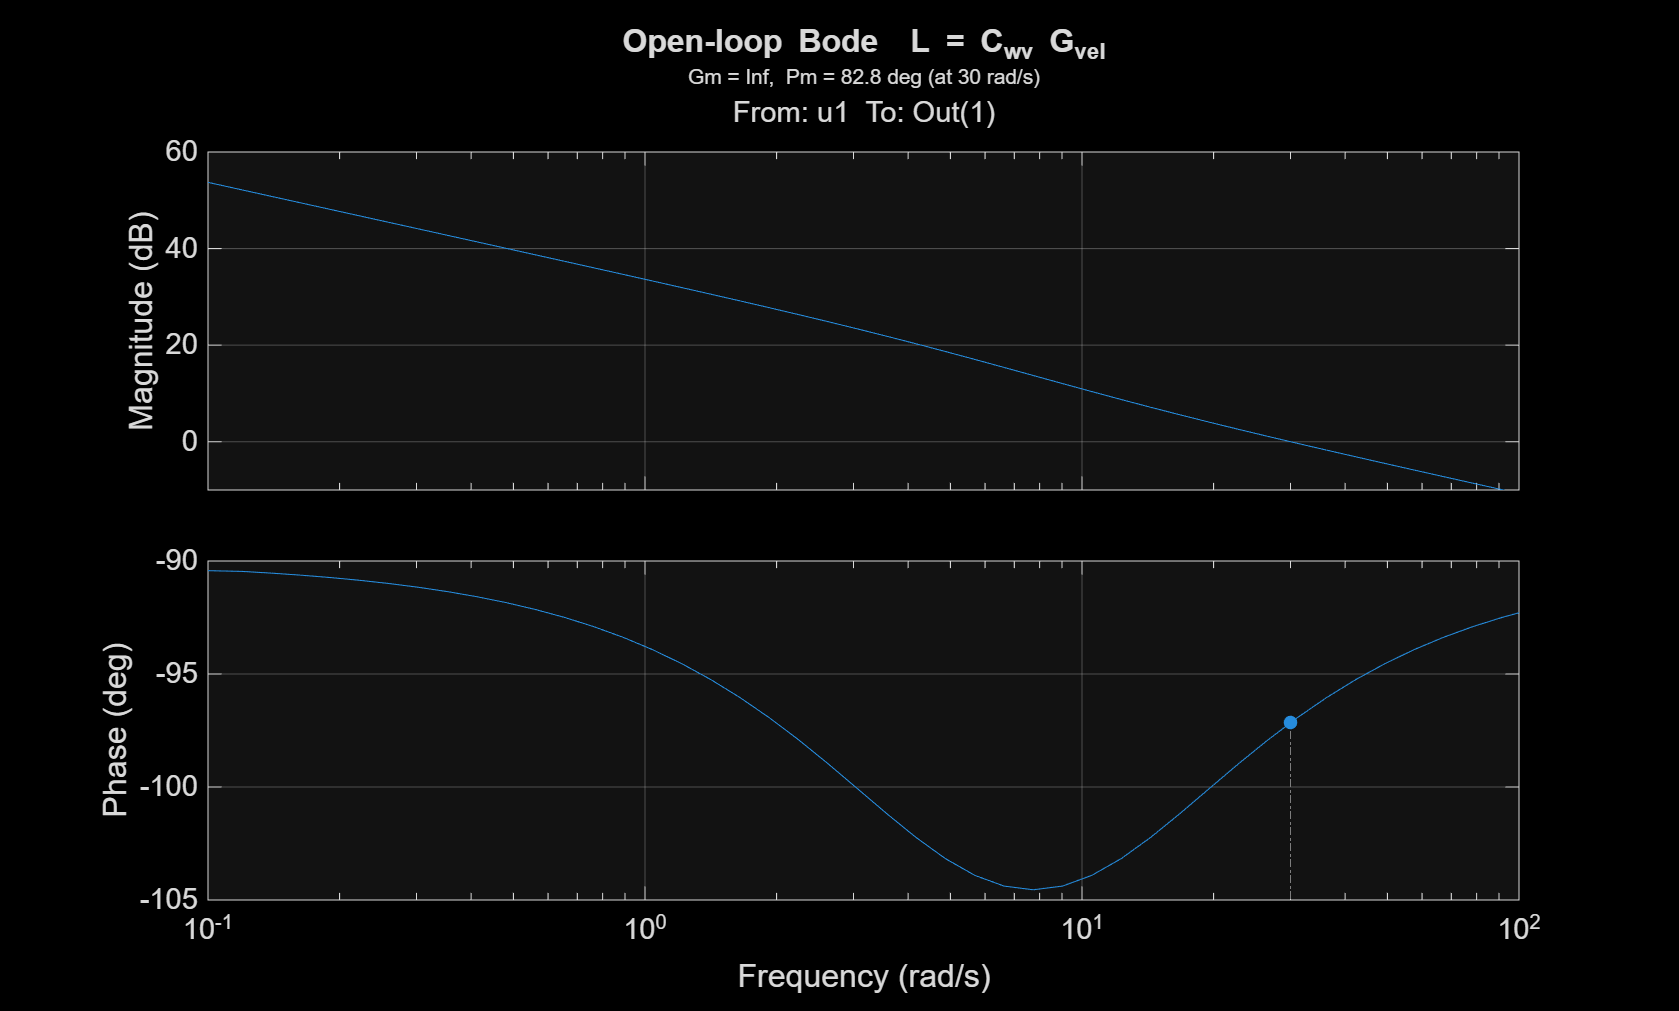
\includegraphics[width=0.8\linewidth]{images/regbot_task1_bode.png}
    \caption{Task~1: Open-loop $L_{wv}$ Bode (Simulink). $\omega_c = 30\,\mathrm{rad/s}$, $\gamma_M = 82.85^{\circ}$, $GM = \infty$.}
    \label{fig:app-task1-bode}
\end{figure}

\begin{figure}[H]
    \centering
    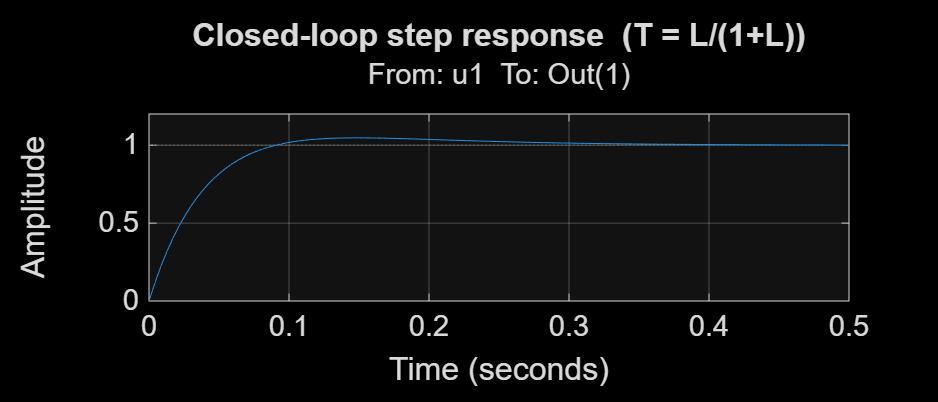
\includegraphics[width=0.8\linewidth]{images/regbot_task1_step.png}
    \caption{Task~1: Closed-loop step response (Simulink).}
    \label{fig:app-task1-sim}
\end{figure}

\begin{figure}[H]
    \centering
    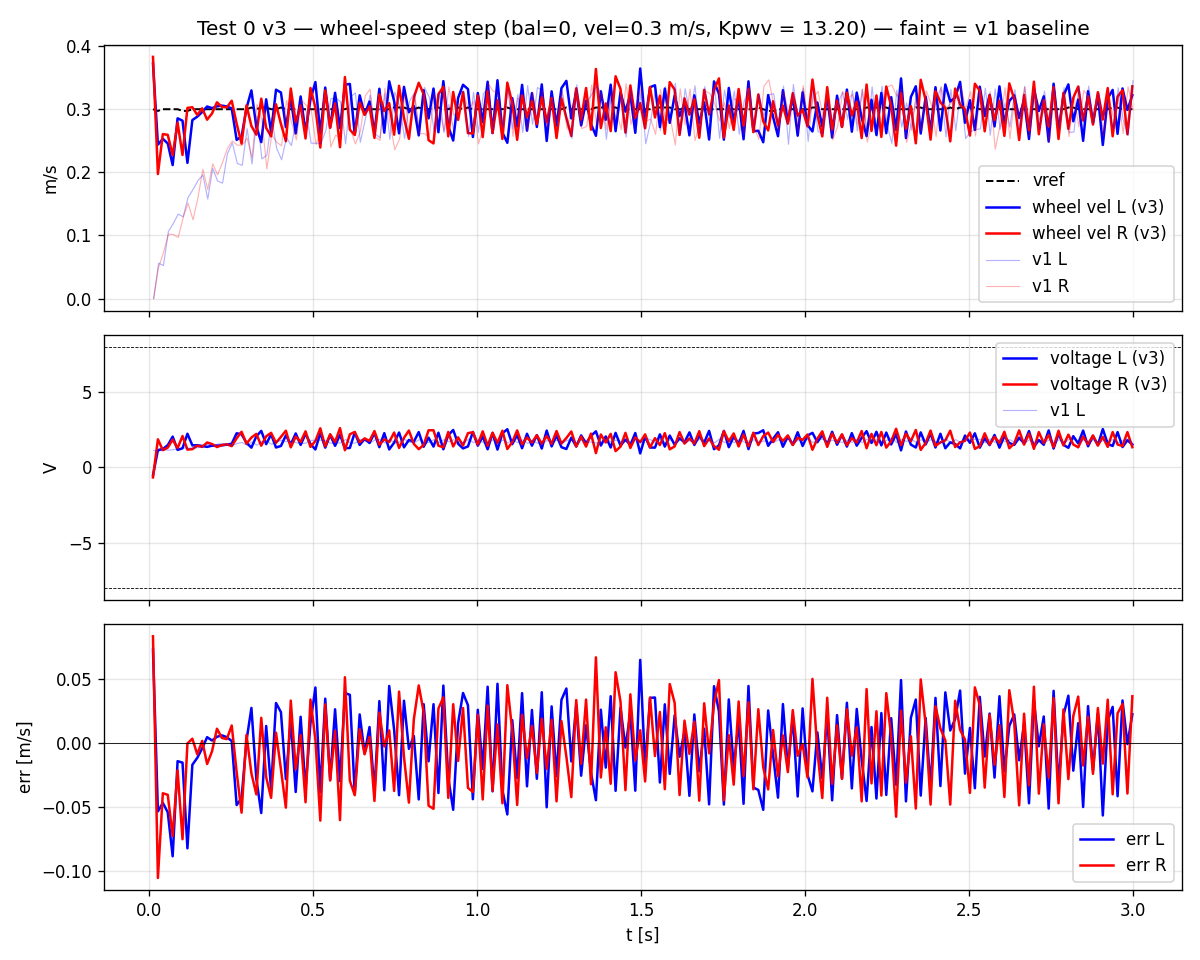
\includegraphics[width=0.8\linewidth]{images/test0_wheel_speed_v3_onfloor_2026-04-22.png}
    \caption{Task~1: Hardware step (Test~0). Mission \texttt{bal=0, vel=0.3, log=15 : time=3}. Rise to $0.27\,\mathrm{m/s}$ in $0.087\,\mathrm{s}$.}
    \label{fig:app-task1-hw}
\end{figure}

\subsection{Task 2 -- Method 2 pre-treatment}
\label{app:task2-method2}
\textit{(expansion of Fig.~\ref{fig:task2_method2} in §\ref{sec:balance})}

\begin{figure}[H]
    \centering
    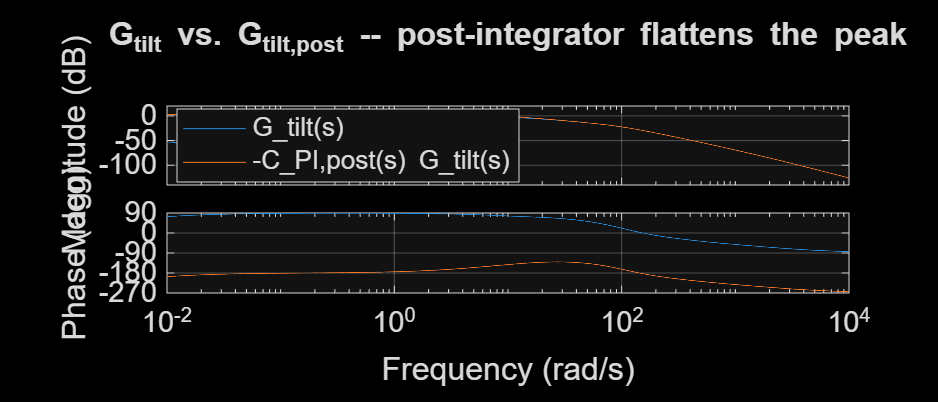
\includegraphics[width=0.8\linewidth]{images/regbot_task2_bode_post.png}
    \caption{Task~2: Bode of $G_{tilt}$ (blue) vs $G_{tilt,\mathrm{post}} = -C_{PI,\mathrm{post}}\,G_{tilt}$ (orange). Magnitude becomes monotonically decreasing after the post-integrator + sign flip.}
    \label{fig:app-task2-bodepost}
\end{figure}

\begin{figure}[H]
    \centering
    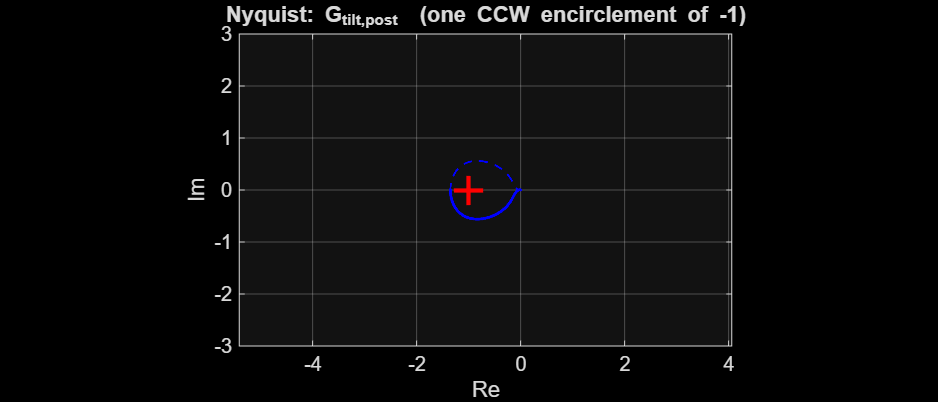
\includegraphics[width=0.55\linewidth]{images/regbot_task2_nyquist_post.png}
    \caption{Task~2: Nyquist of $G_{tilt,\mathrm{post}}$. Exactly one CCW encirclement of $(-1,0)$ -- the visual proof that $Z = N + P = -1 + 1 = 0$ and Method~2 has stabilised the plant.}
    \label{fig:app-task2-nyquist}
\end{figure}

\subsection{Task 2 -- Balance verification}
\label{app:task2-verify}
\textit{(expansion of Fig.~\ref{fig:task2-verify} in §\ref{sec:balance})}

\begin{figure}[H]
    \centering
    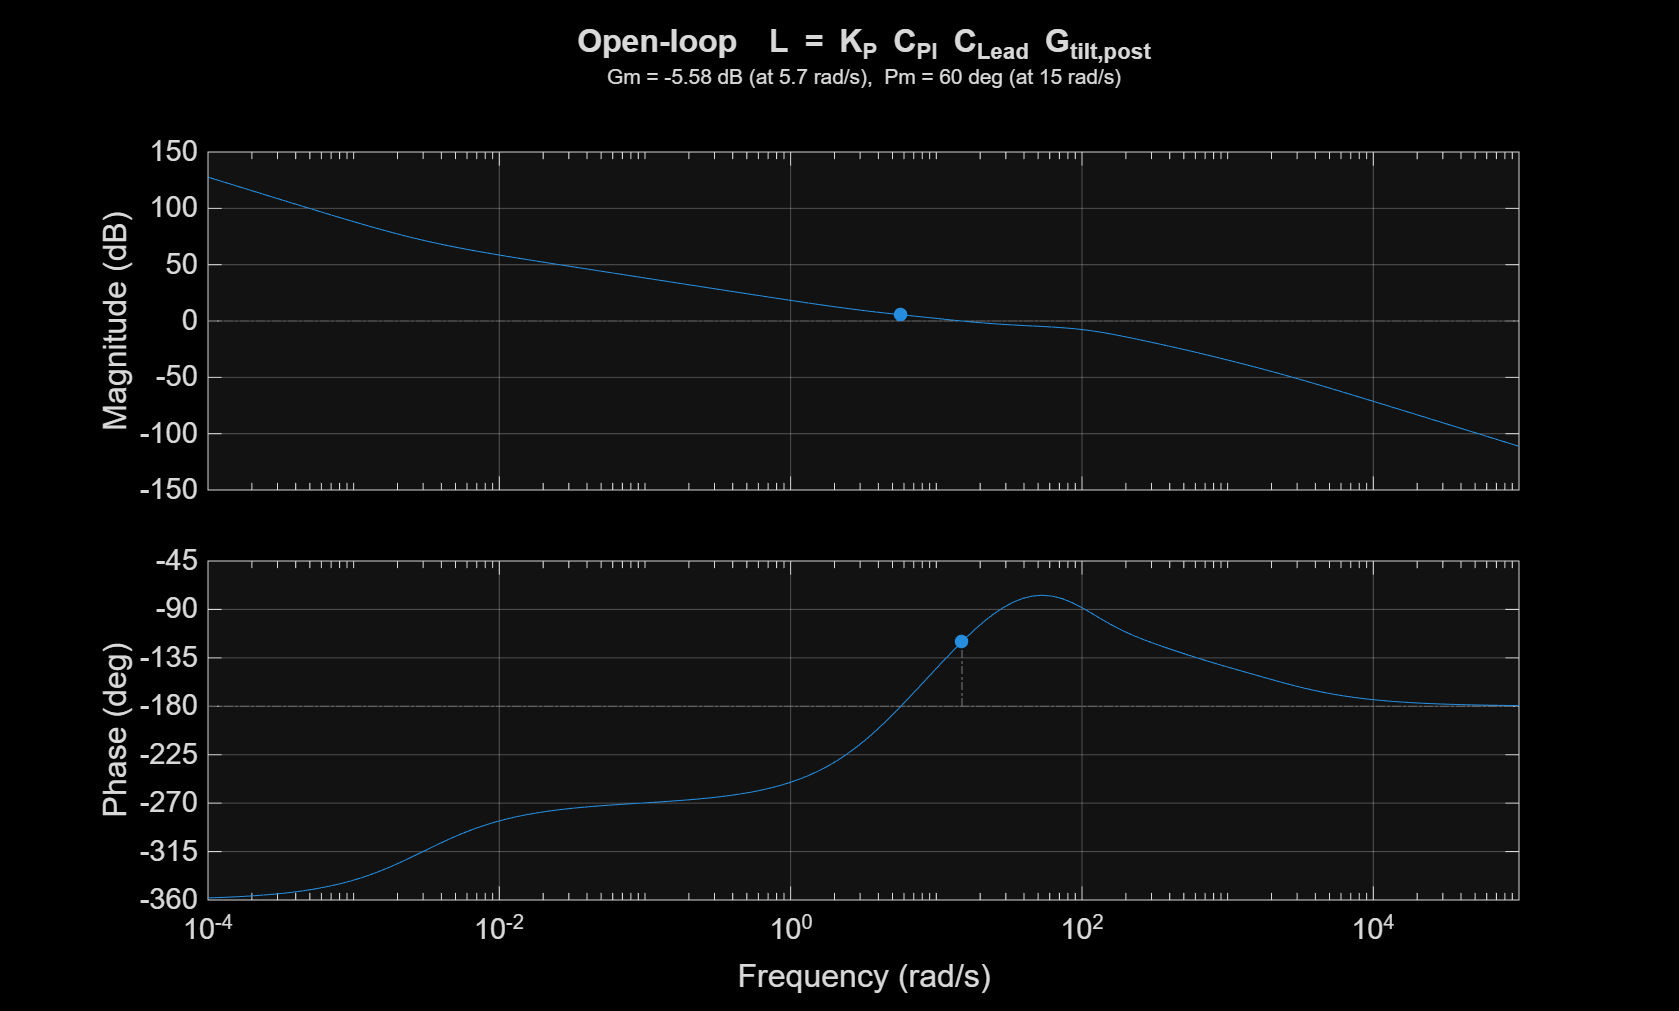
\includegraphics[width=0.8\linewidth]{images/regbot_task2_loop_bode.png}
    \caption{Task~2: Open-loop $L_{\mathrm{tilt}} = K_P\,C_{PI}\,C_{\mathrm{Lead}}\,G_{tilt,\mathrm{post}}$ Bode (Simulink). $\omega_c = 15.00\,\mathrm{rad/s}$, $\gamma_M = 60.00^{\circ}$, $GM = -5.58\,\mathrm{dB}$ (negative GM is the lower bound on $|K|$ for unstable plants).}
    \label{fig:app-task2-bode}
\end{figure}

\begin{figure}[H]
    \centering
    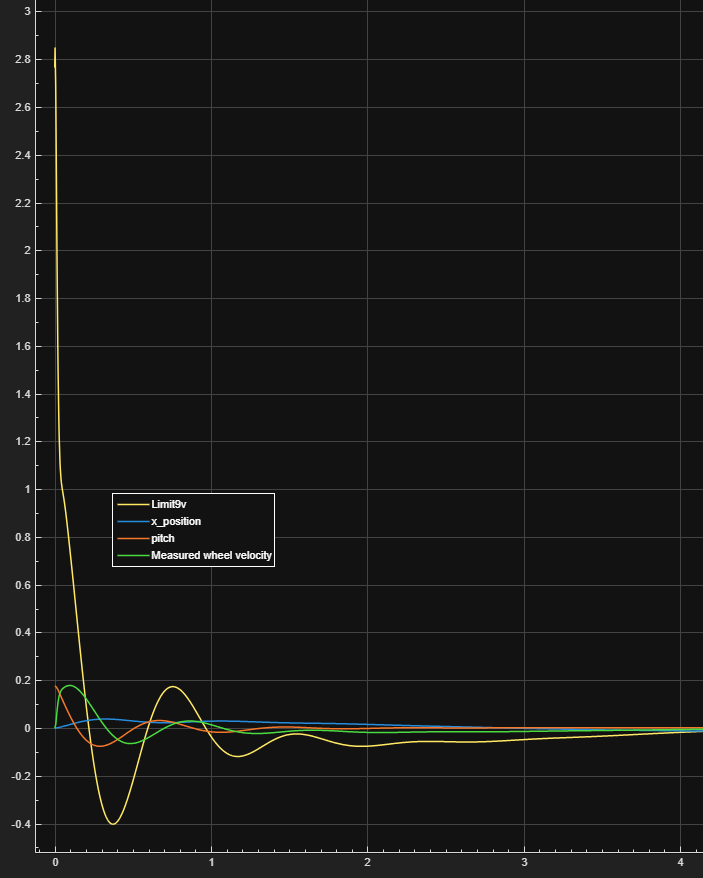
\includegraphics[width=0.8\linewidth]{images/regbot_task2_sim_recovery_10deg_v3.png}
    \caption{Task~2: Simulink full-cascade recovery from a $10^{\circ}$ tilt push. Traces: limited motor voltage (yellow, $\pm 9\,\mathrm{V}$), $x$ position (blue), pitch (red), measured wheel velocity (green). Pitch returns to zero within $\sim 2\,\mathrm{s}$; the linear-model IC release through $S = 1/(1+L)$ predicts $1.34\,\mathrm{s}$ 2\,\%-settle and $\sim 6.6^{\circ}$ peak undershoot.}
    \label{fig:app-task2-sim}
\end{figure}

\begin{figure}[H]
    \centering
    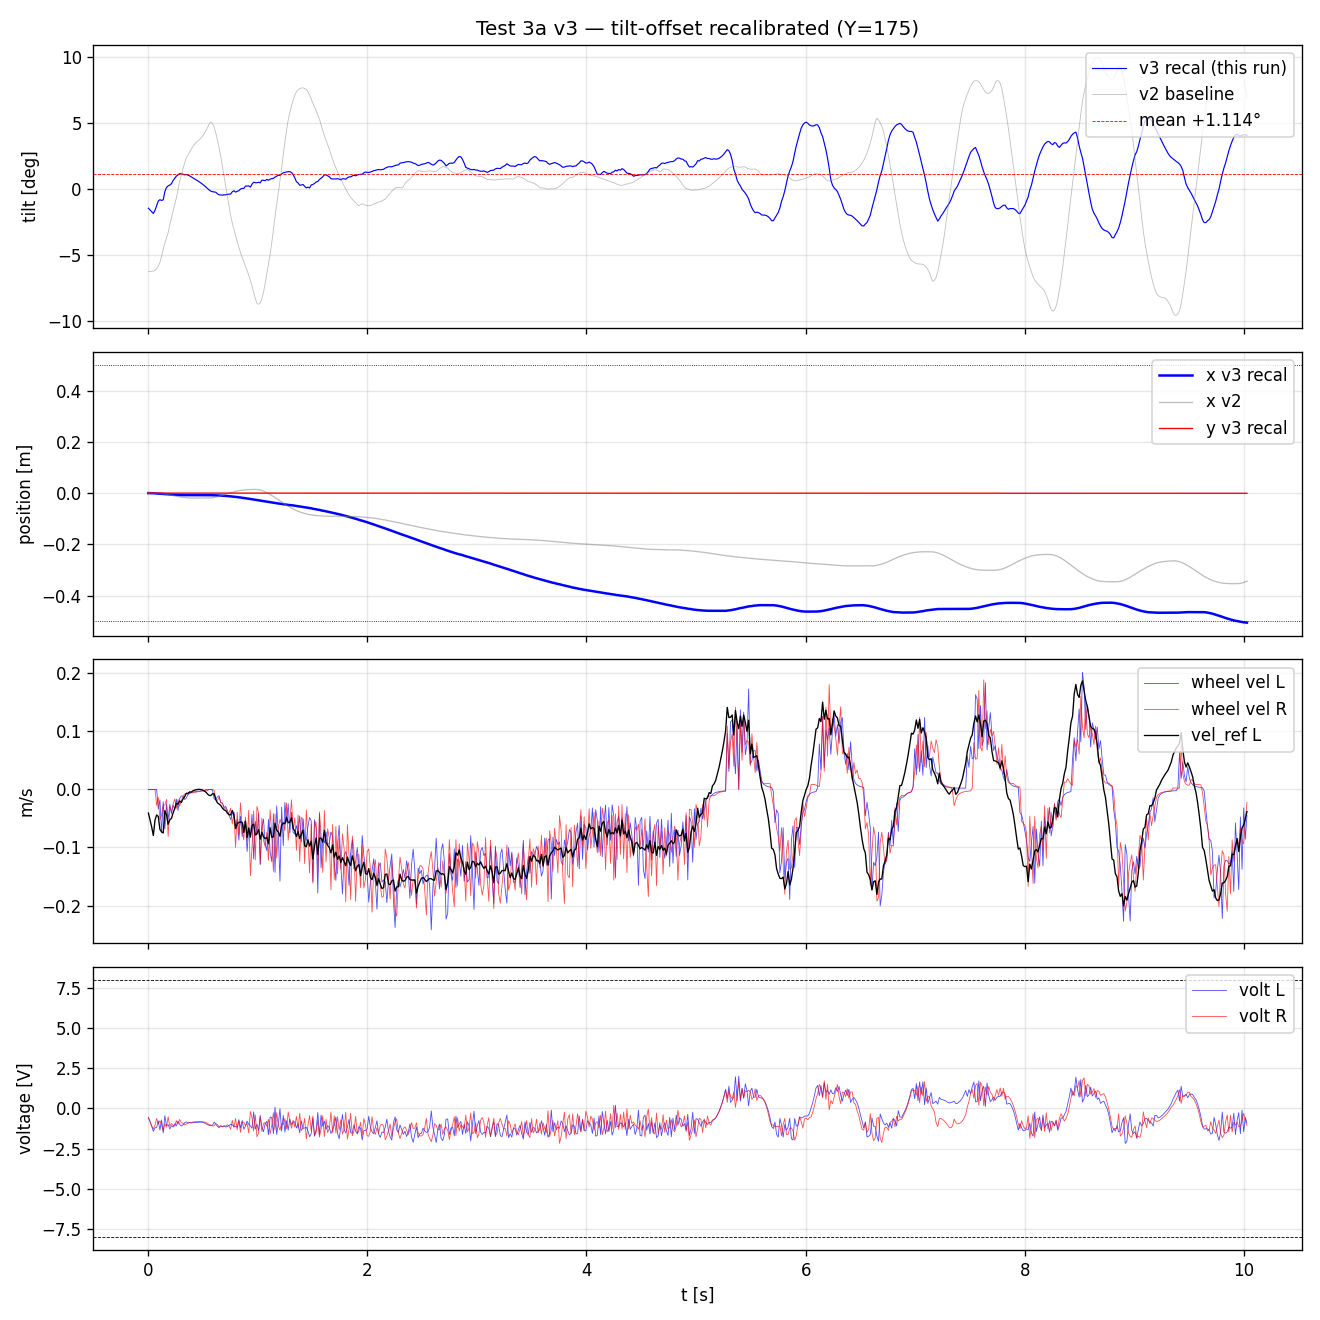
\includegraphics[width=0.8\linewidth]{images/test3a_balance_rest_v3_onfloor_2026-04-22.png}
    \caption{Task~2: Hardware balance hold (Test~3a). Mission \texttt{vel=0, bal=1, log=15 : time=10}. Drift $0.343\,\mathrm{m}$ over $10\,\mathrm{s}$ (spec $\leq 0.5$ \checkmark).}
    \label{fig:app-task2-hw}
\end{figure}

\subsection{Task 3 -- Velocity verification}
\label{app:task3-verify}
\textit{(expansion of Fig.~\ref{fig:task3-verify} in §\ref{sec:velocity})}

\begin{figure}[H]
    \centering
    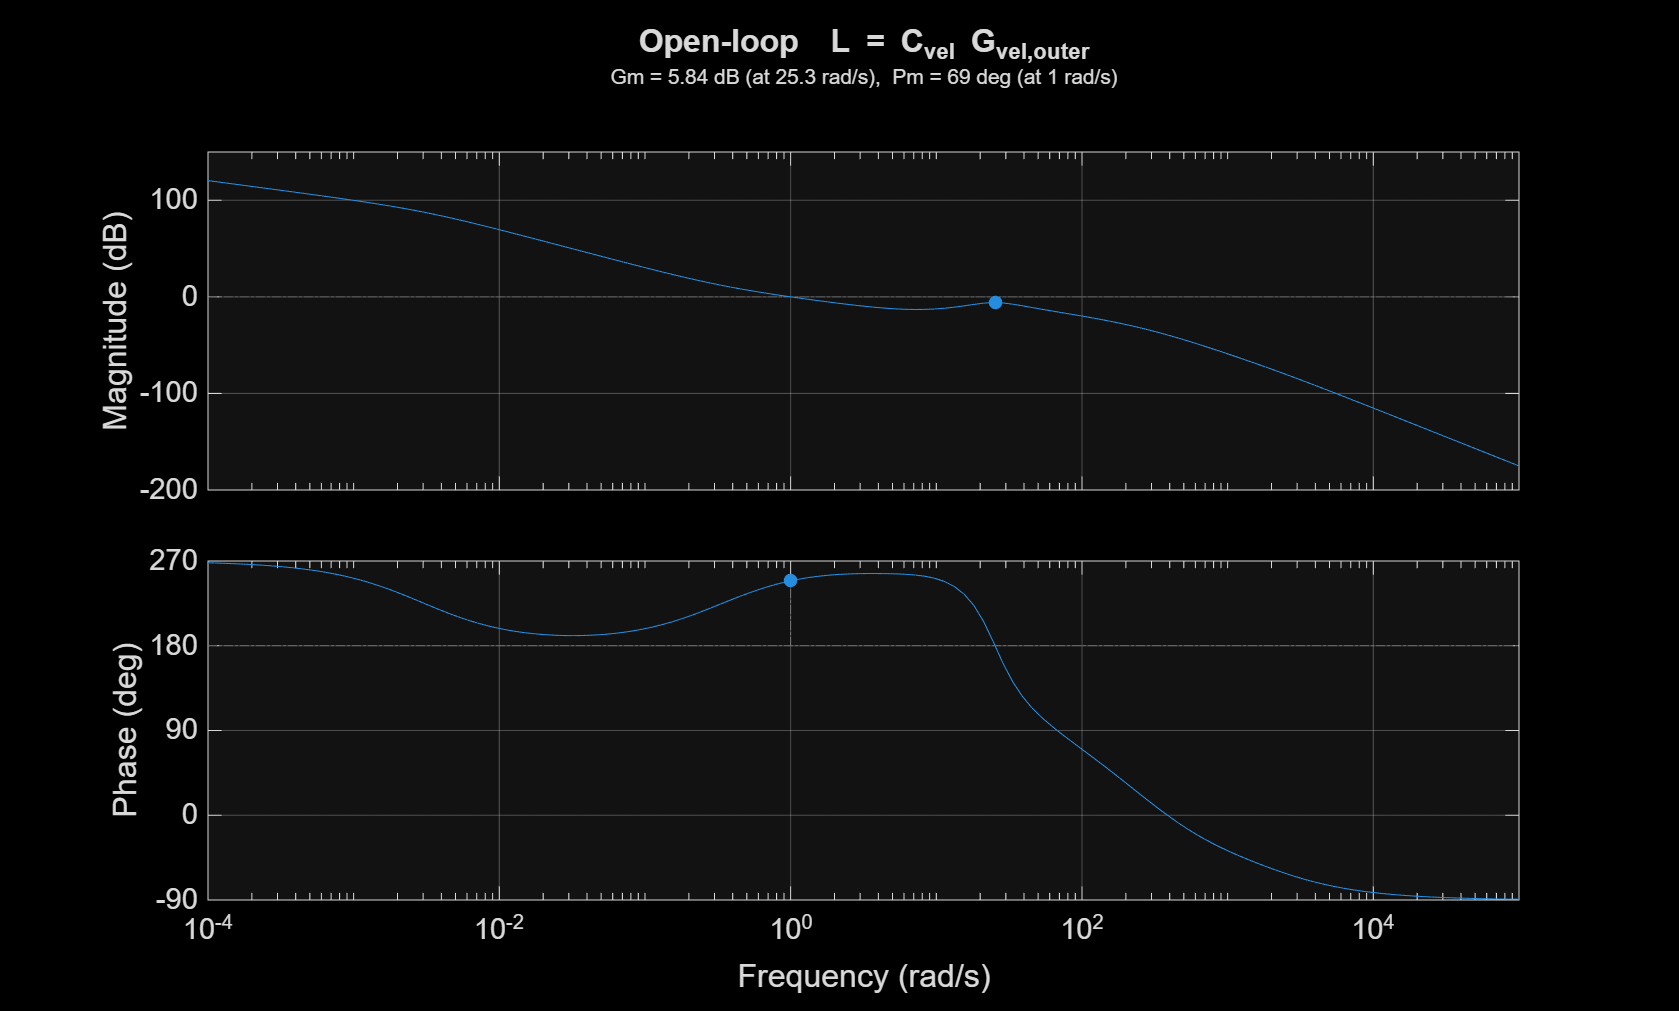
\includegraphics[width=0.8\linewidth]{images/regbot_task3_loop_bode.png}
    \caption{Task~3: Open-loop $L_{\mathrm{vel}}$ Bode (Simulink). $\omega_c = 1.00\,\mathrm{rad/s}$, $\gamma_M = 68.98^{\circ}$, $GM = 5.84\,\mathrm{dB}$.}
    \label{fig:app-task3-bode}
\end{figure}

\begin{figure}[H]
    \centering
    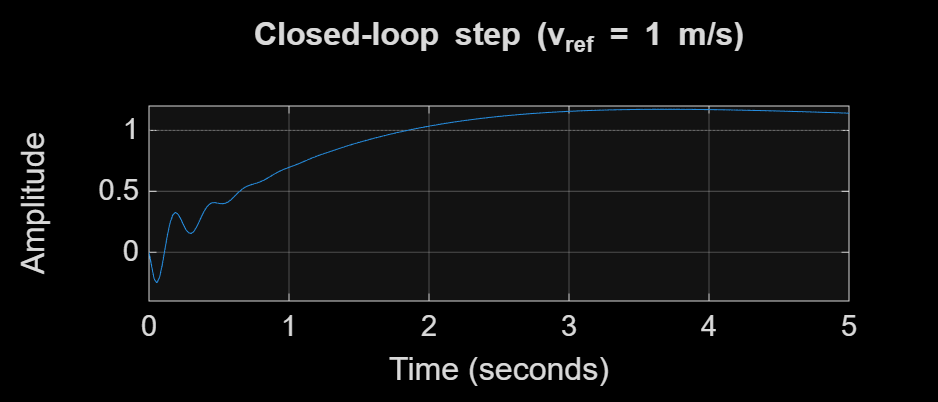
\includegraphics[width=0.8\linewidth]{images/regbot_task3_step.png}
    \caption{Task~3: Closed-loop step (Simulink), $v_{\mathrm{ref}} = 1\,\mathrm{m/s}$.}
    \label{fig:app-task3-sim}
\end{figure}

\begin{figure}[H]
    \centering
    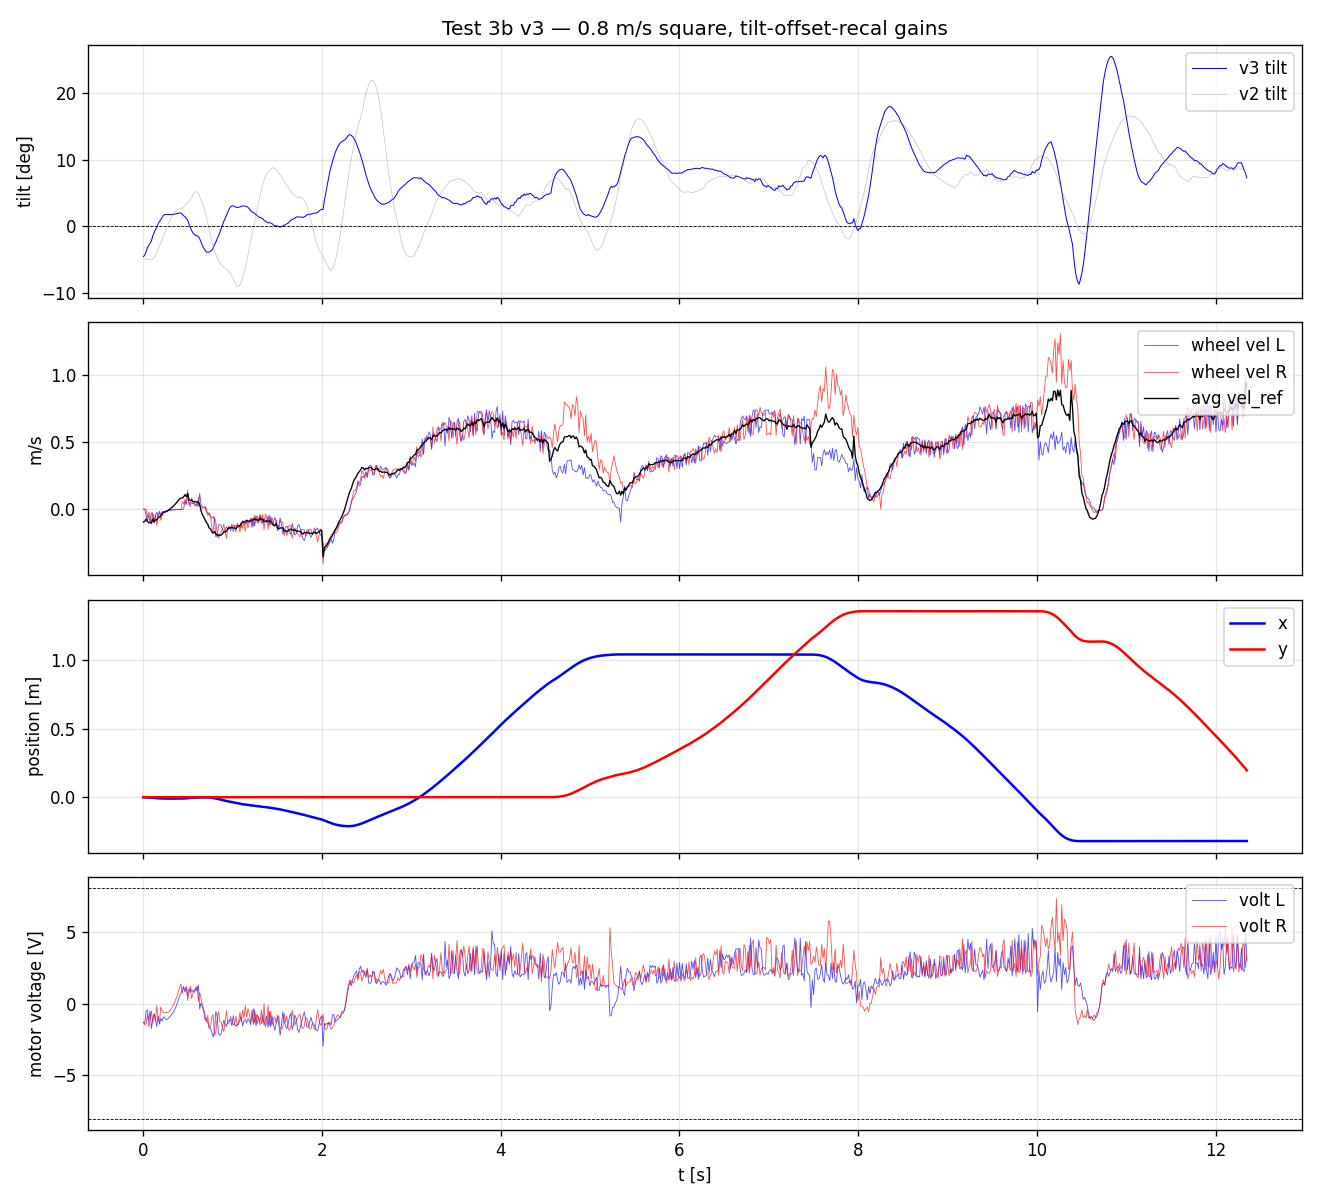
\includegraphics[width=0.8\linewidth]{images/test3b_timeseries_v3_onfloor_2026-04-22.png}
    \caption{Task~3: Hardware time series (Test~3b). Mission $4\times$ \texttt{vel=0.8 : dist=1 ; vel=0.8, tr=0.2 : turn=90}. Peak tilt $+25.5^{\circ}$ at corners, peak motor voltage $7.31\,\mathrm{V}$.}
    \label{fig:app-task3-hw}
\end{figure}

\subsection{Task 3 -- XY trajectory}
\label{app:task3-xy}
\textit{(expansion of Fig.~\ref{fig:task3-xy} in §\ref{sec:velocity})}

\begin{figure}[H]
    \centering
    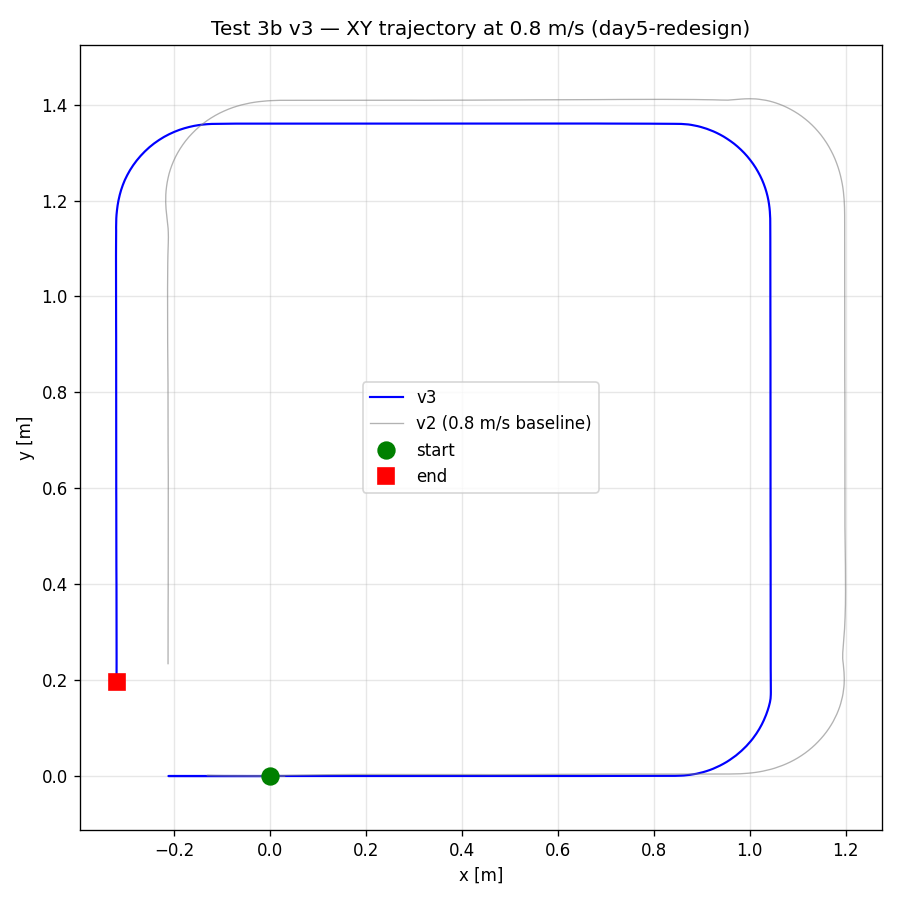
\includegraphics[width=0.7\linewidth]{images/test3b_xy_v3_onfloor_2026-04-22.png}
    \caption{Test~3b XY trajectory at $0.8\,\mathrm{m/s}$ ($1\,\mathrm{m}$ sides, $0.2\,\mathrm{m}$ corner radius). Cumulative heading $359.8^{\circ}$ after one square lap (four $90^{\circ}$ turns).}
    \label{fig:app-task3-xy}
\end{figure}

\subsection{Task 4 -- Position verification}
\label{app:task4-verify}
\textit{(expansion of Fig.~\ref{fig:task4-verify} in §\ref{sec:position})}

\begin{figure}[H]
    \centering
    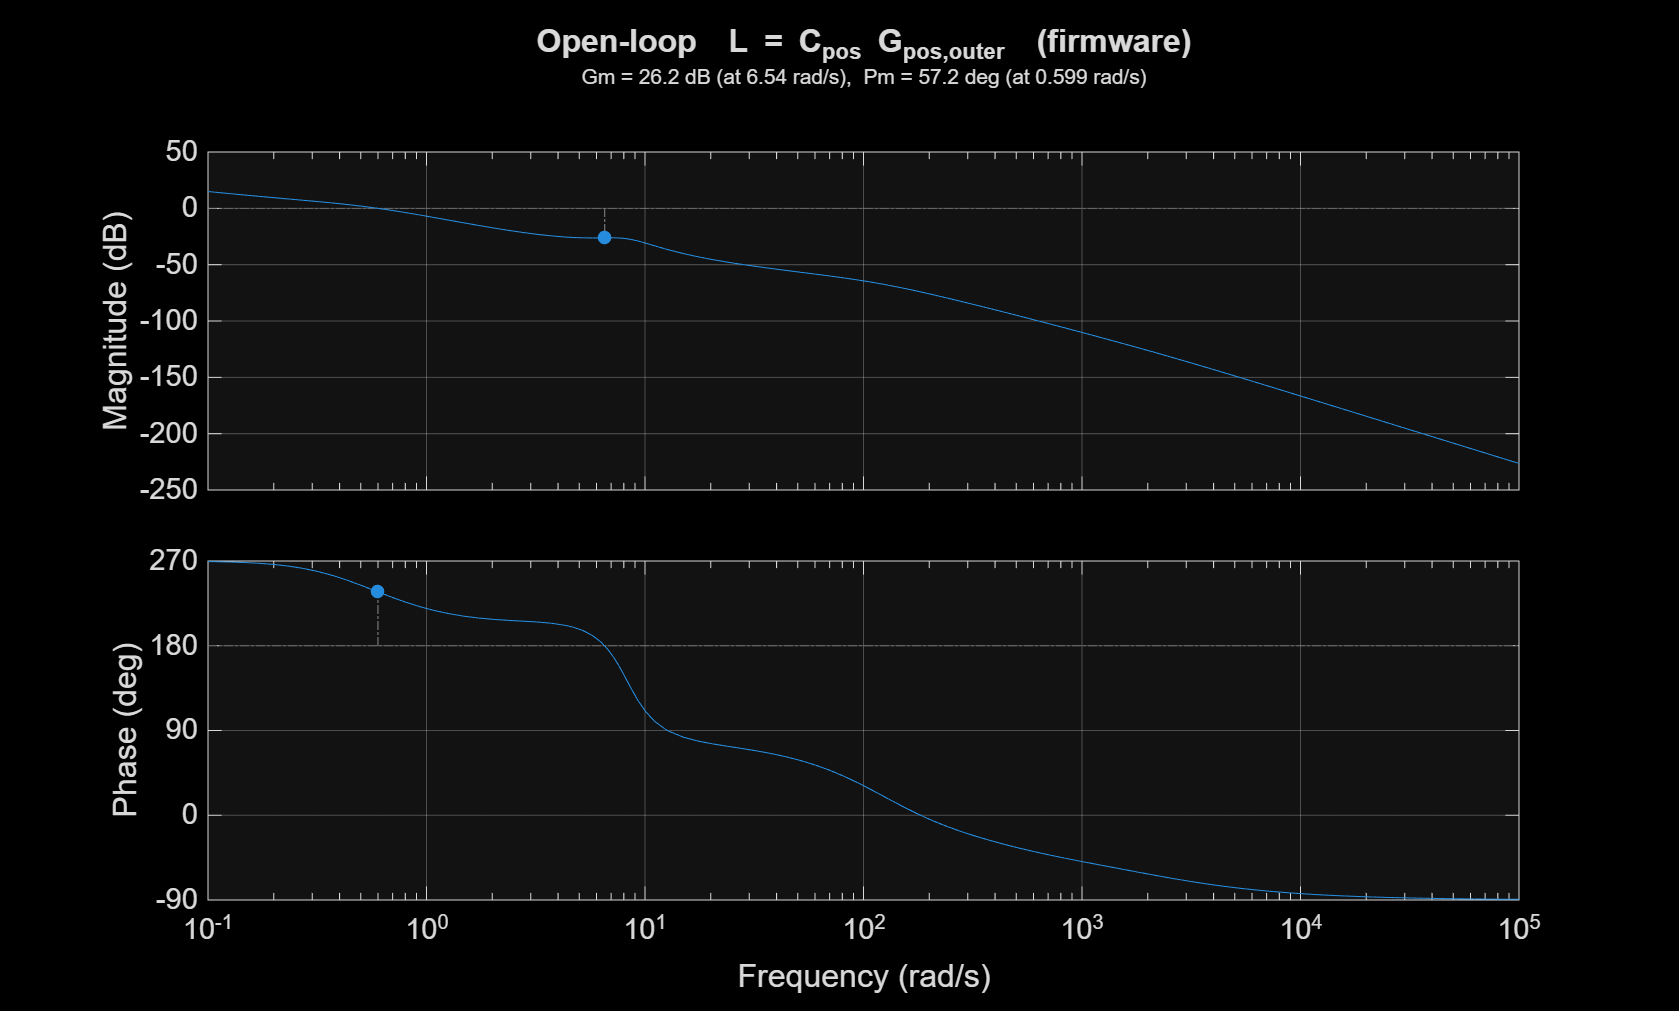
\includegraphics[width=0.8\linewidth]{images/regbot_task4_loop_bode.png}
    \caption{Task~4: Open-loop $L_{\mathrm{pos}}$ Bode (Simulink, firmware controller with Lead dropped). $\omega_c = 0.60\,\mathrm{rad/s}$, $\gamma_M = 57.18^{\circ}$, $GM = 26.20\,\mathrm{dB}$.}
    \label{fig:app-task4-bode}
\end{figure}

\begin{figure}[H]
    \centering
    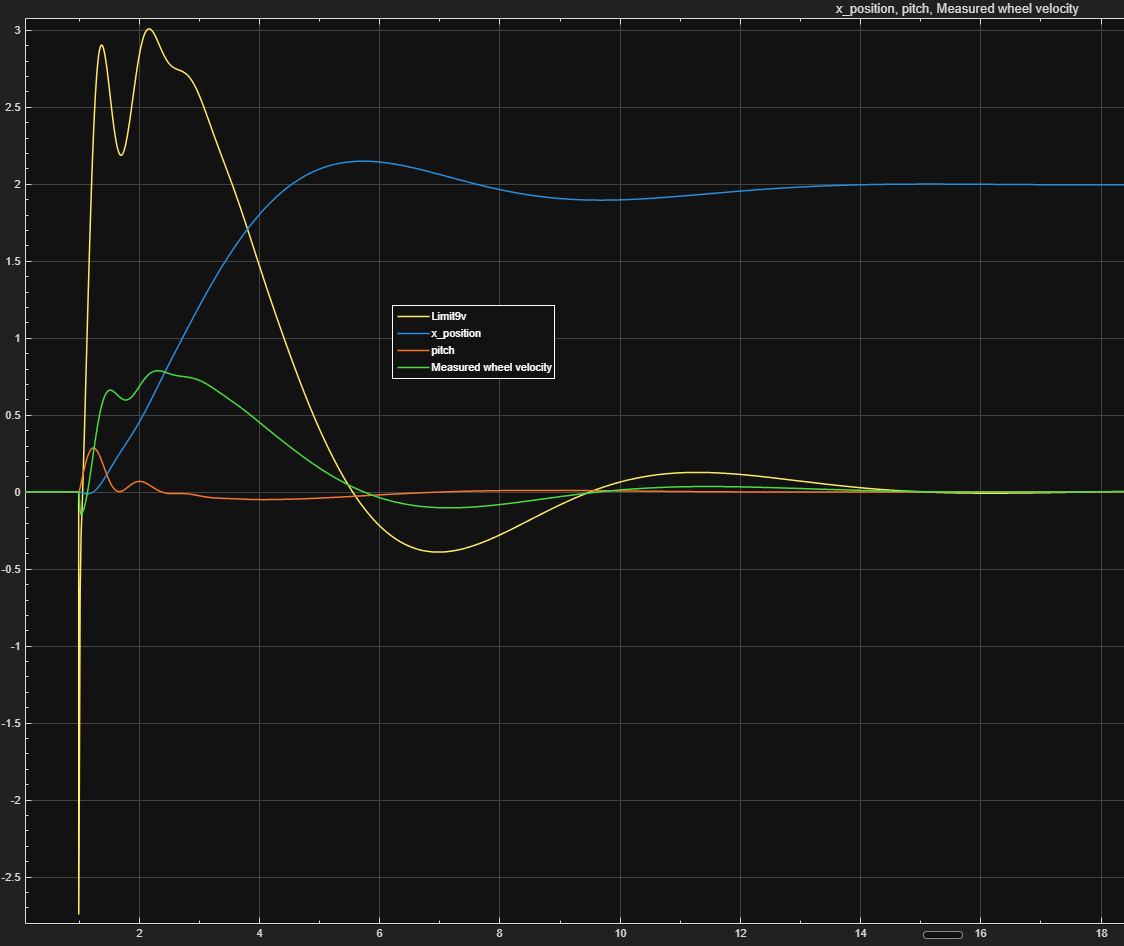
\includegraphics[width=0.8\linewidth]{images/regbot_task4_sim_step_v3.png}
    \caption{Task~4: Simulink full-cascade 2\,m step at $t = 1\,\mathrm{s}$. Position (blue) reaches $2\,\mathrm{m}$; intermediate tilt and velocity traces visible.}
    \label{fig:app-task4-sim}
\end{figure}

\begin{figure}[H]
    \centering
    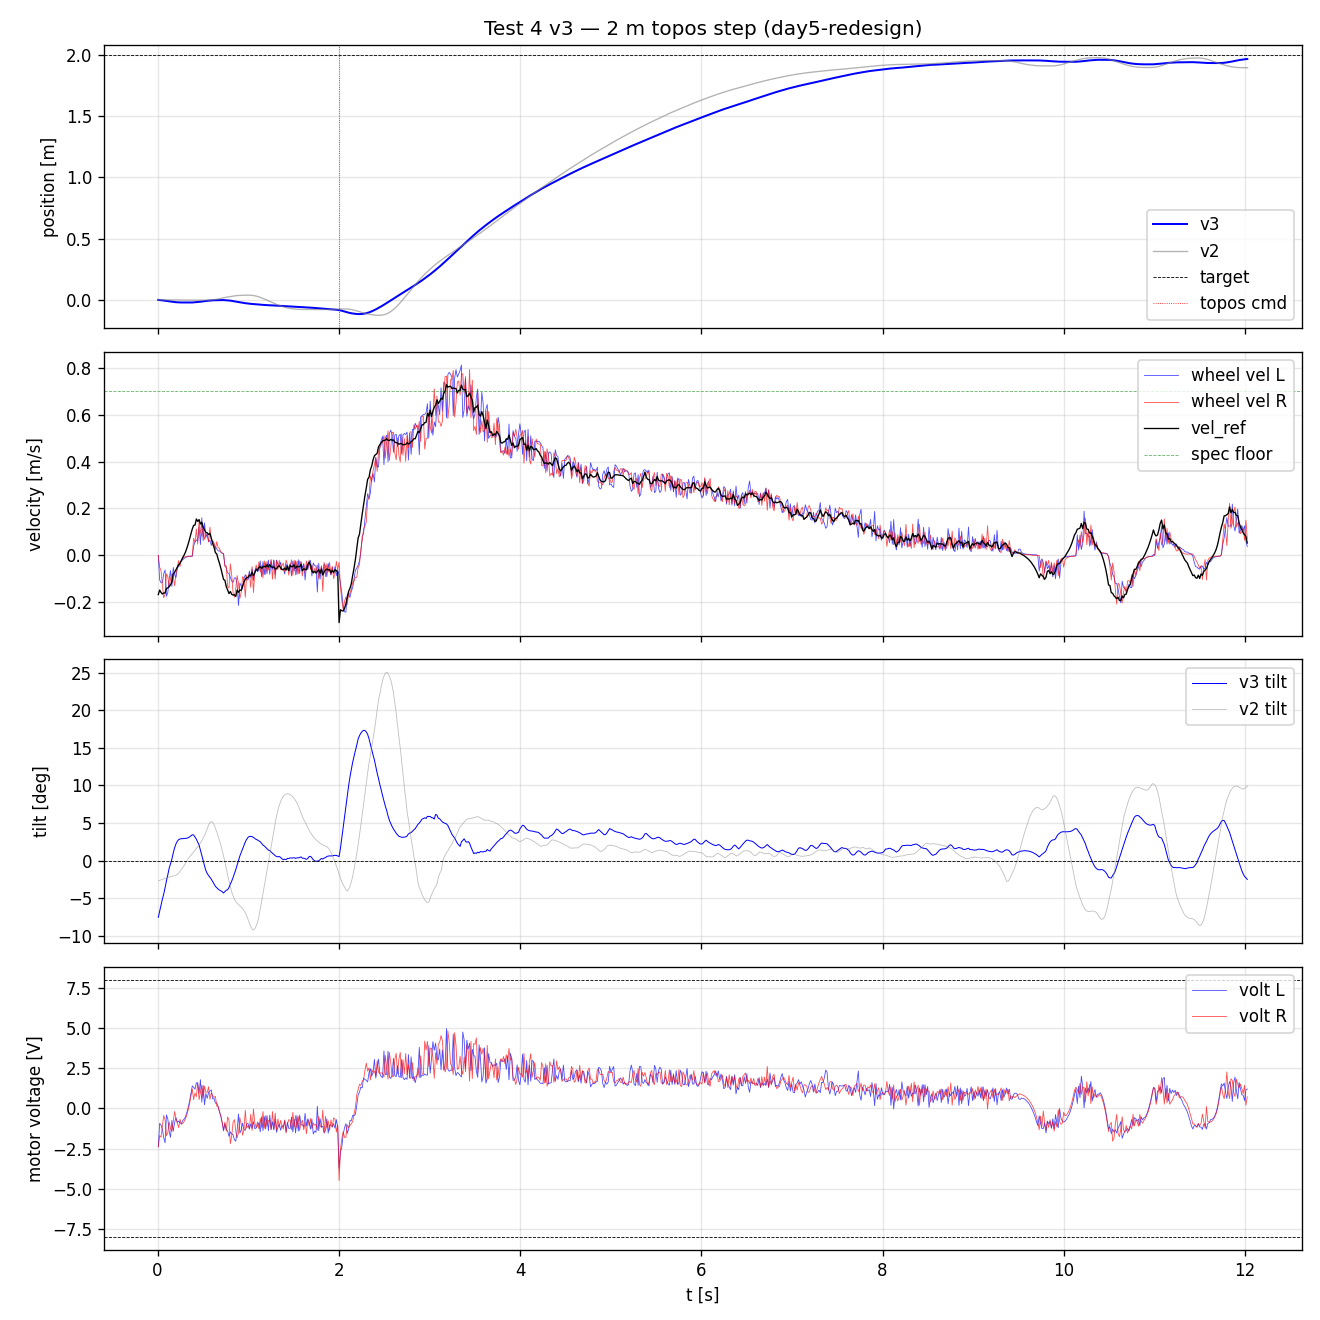
\includegraphics[width=0.8\linewidth]{images/test4_position_2m_v3_onfloor_2026-04-22.png}
    \caption{Task~4: Hardware 2\,m step (Test~4). Mission \texttt{vel=0, bal=1, log=15 : time=2 ; topos=2, vel=1.2 : time=10}. Final position $1.964\,\mathrm{m}$, peak $v = 0.79\,\mathrm{m/s}$.}
    \label{fig:app-task4-hw}
\end{figure}
